\documentclass[thesis.tex]{subfiles}
\begin{document}

\chapter{Methodology}\label{chap:basics}

In this chapter we describe in detail how each step of our proposed pipeline is realized. In the first step of the pipeline we obtain cross-sections by going along the centerlines in the volume data. Then, we extract the contours of the TL and FL from the obtained cross-sections. In the third step of the pipeline we represent the extracted contours using chain codes. We then apply a fourier transform on the chain codes to obtain EFDs. In the fifth step we then use the EFDs to approximate the lumen shapes and correct the overlapping contours that might occur. The result is then be used for visualization, rendering, and interpolation. We also add a vessel wall around the recontructed and corrected contours. An overview of this pipeline is shown in Figure \ref{fig:pipeline}. We demonstrate all methods on a phantom data set thoughout this chapter. 

\begin{center}
\begin{tikzpicture}[node distance = 3cm, auto] \label{fig:pipeline}

    % Place nodes
    \node [block] (init) {Obtain cross-sections};
    \node [cloud, left of=init] (expert) {expert};
    \node [block, below of=init] (contours) {Extract contours};
    \node [block, below of=contours] (chaincode) {Convert contours to chain codes};
    \node [block, below of=chaincode] (efds) {Compute EFDs};
    \node [decision, below of=efds, node distance=4cm] (decide) {Cross-sections obtained with TCL ?};
    \node [block, below of=decide, node distance=4cm] (overlap) {Correct overlapping contours};
	\node [block, below of=overlap] (vesselwall) {Create vessel wall};
	\node [block, below of=vesselwall] (use) {Use EFDs for rendering etc.};
    % Draw edges
    \path [line] (init) -- (contours);
    \path [line] (contours) -- (chaincode);
    \path [line] (chaincode) -- (efds);
	\path [line] (efds) -- (decide);
	\path [line] (overlap) -- (vesselwall);
	\path [line] (vesselwall) -- (use);
    %\path [line] (decide) -- node {no} (use);
    \path [line] (decide) -- node {yes}(overlap);
    %\path [line,dashed] (expert) -- (init);
\end{tikzpicture}
\end{center}


\section{Obtaining Cross-Sections}
In this step of the pipeline we describe how cross-sections are obtained from the provided volume data. Each dataset of the provided data contains three centerlines, the centerline of the FL, the centerline of the TL , and the TCL. The TCL interpolates points that lie between the centerlines of the TL and FL. All centerlines are modeled by interpolating B-Splines. To obtain cross-sections, we go along a centerline using a fixed step size and compute a local coordinate frame at each position that we visit on the centerline. The step size is computed by dividing the length of the centerline by the number of desired cross-sections, which is a parameter the user can specify. This ensures that each lumen is represented by the same amount of cross-sections. Each local coordinate frame consist of two 3-dimensional vectors, which are orthogonal to the centerline at the centerline position they were obtained. The two vectors define the x- and y-axis of the cross-section in the 3-dimensional space of the volume data. Starting from the centerline position we sample the volume in the directions of the positive and negative x- and y-axes of the cross-section. By doing this we obtain the positions of the cross-section pixels in the 3-dimensional space of the volume data. The positive and negative x- and y-axes are used because we want the centerline to be in the center of the cross-section. The obtained 3-dimensional positions have floating point precision and are truncated to their integer, which corresponds to the the position of a voxel in the volume. The final intensity of a pixel in the cross-section is then obtained by trilinear interpolation of the non-zero values of this voxel and the 7 neighboring voxels that form a volume cell.  

A screenshot of the centerlines of our phantom data set is shown in Figure \ref{fig:obliqueslices}. The figure also shows a cross-section obtained from each centerline using the same offset. Even though the same offset was used, all three cross-sections are different. The cross-section from the TL centerline and TCL in the figure are oriented differently and it can be seen that the cross-section from the TL is not orthogonal to the TCL and the other way around. The cross-section from the FL centerline was obtained using the same offset as the other cross-sections, but is on a completely different position in the volume. This is because the FL centerline is shorter than the other centerlines in the volume, which results in a smaller step size when going along the centerline. 

\begin{figure}
	\begin{subfigure}[t]{0.45\textwidth}
		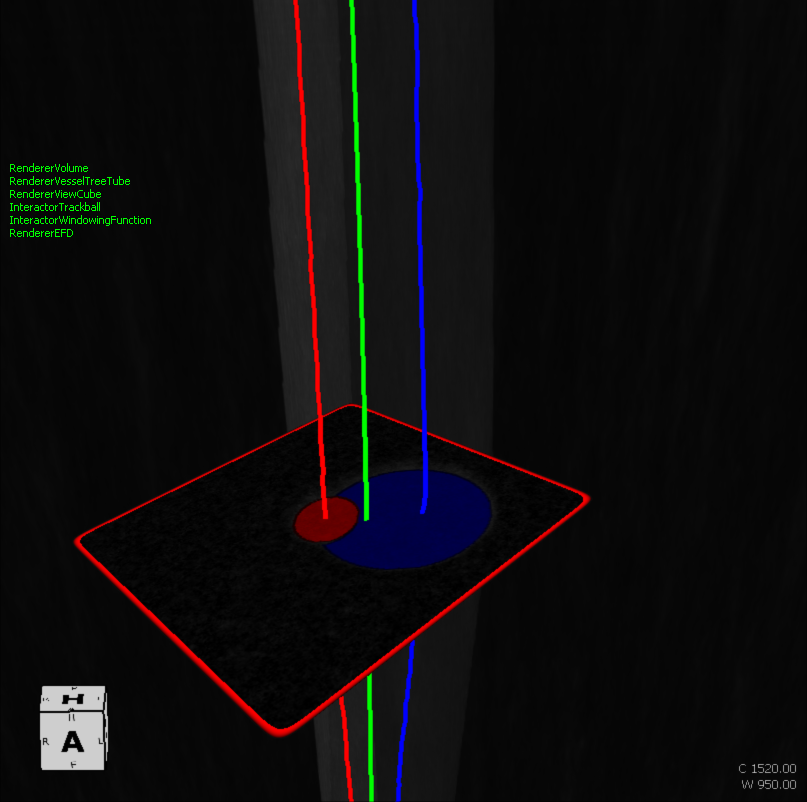
\includegraphics[width=\textwidth]{obliqueslices_tl_615.PNG}
	\caption{}		
	\end{subfigure}
\hspace{0.05\textwidth}
	\begin{subfigure}[t]{0.45\textwidth}
		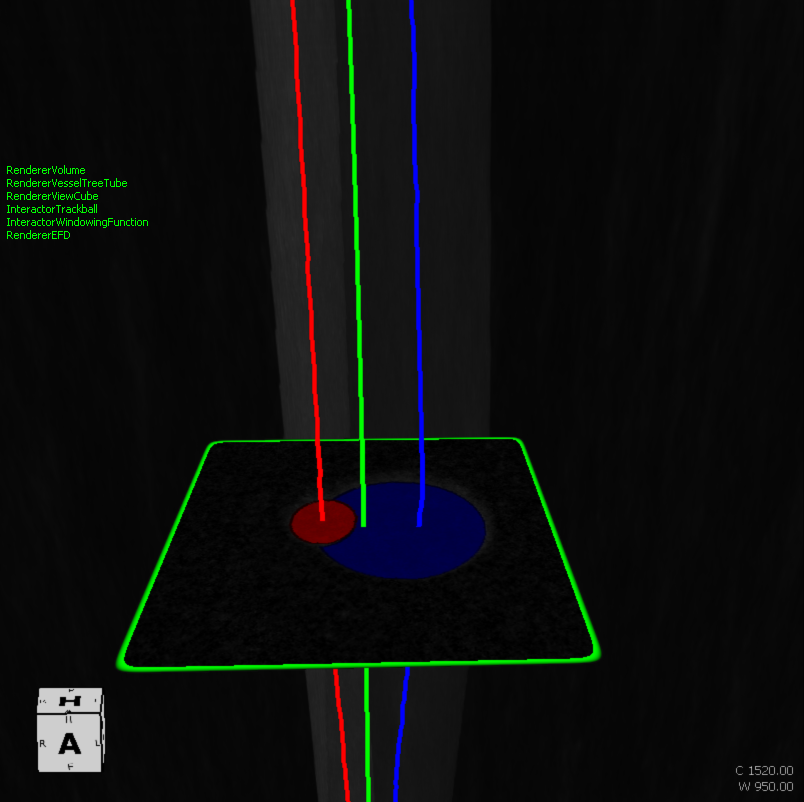
\includegraphics[width=\textwidth]{obliqueslices_tcl_615.PNG}		
\caption{}	
	\end{subfigure}
\centering
\begin{subfigure}[t]{0.45\textwidth}
		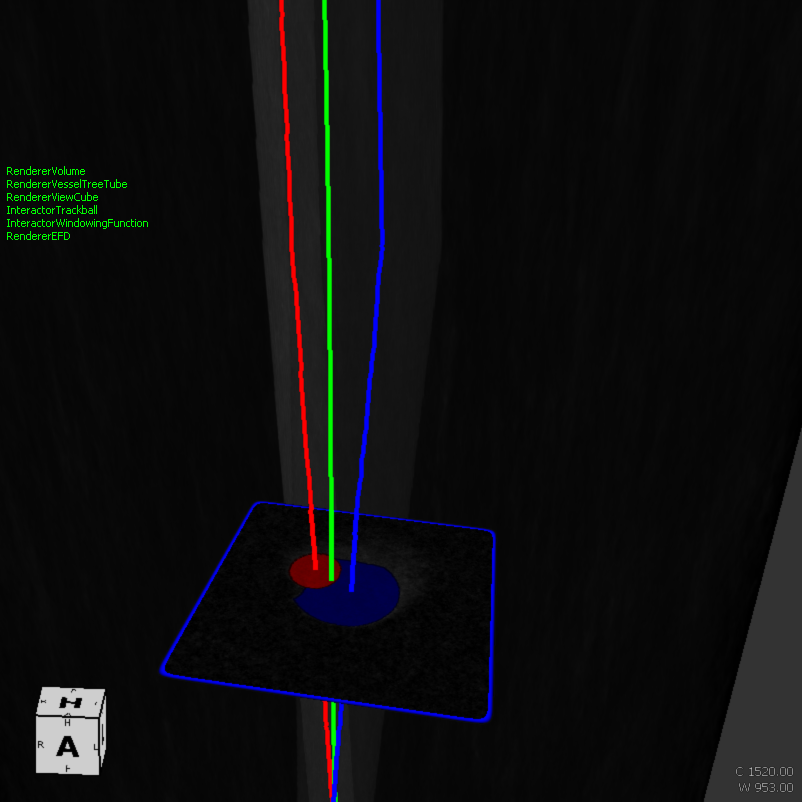
\includegraphics[width=\textwidth]{obliqueslices_fl_615.PNG}		
\caption{}	
	\end{subfigure}
	\caption{The three centerlines of our phantom dataset. The TL centerline, TCL, and FL centerline are colored red, green, and blue respectively. A cross-section is shown for each centerline. The cross-sections are orthogonal to their corresponding centerline, but not necessarily to other centerlines. That is why the cross-section of the TL and TCL look slightly different, even though the same offset was used. The cross-section of the FL also uses the same offset, but because the FL centerline is shorter than the TL centerline and the TCL, the cross-section apppears on a completly different position.}
\label{fig:obliqueslices}
\end{figure}



By default we use the TCL to obtain cross-sections, but the user can also choose to use the centerlines of the TL and FL instead. We chose the TCL as default, because the obtained cross-sections are easier to use in the other steps of the pipeline.
In the following we describe problems that can occur when obtaining cross-sections and how we solved or avoided them. 

\subsection{Problems when obtaining cross-sections}
\label{problems_crosssections}
\textbf{Centerline positions with high curvature} 

On positions of the centerline with high curvature, overlapping cross-sections can occur. They can be problematic, because some surface rendering algorithms such as marching cubes work by connecting points from consecutive cross-sections. However, when cross-sections overlap, inner structures within the surface occur. These inner structures make the surface useless for severeal appplications. When simulating the flow of blood within the lumen for example, the result is influenced by the inner structures. Therefore, only surfaces without inner structures are desired. A possible solution was proposed by the authors of \cite{wu2010curvature}. They propose to use an adaptive step size that depends on the gaussian curvature of the centerline to bi-directionally down-sample the centerline, before obtaining cross-sections. This ensures that cross-sections are far apart in regions of high curvature. 

We avoided this problem by not storing the correspondence of contour pixels to their cross-section. This means we interpret the extracted contours as a point cloud.

Another problem caused by high curvature of the centerline is the appearance of a lumen at several positions in the cross-section. Figure \ref{fig:overlappingCase} shows a cross-section near the aortic arch, where the curvature is relatively high. In the figure the TL is marked red and the FL is marked blue. As can be seen in the figure, the TL appears at two positions in the cross-section. The result of extracting the lumen contours from such a cross-section is shown in Figure \ref{fig:overlappingCrossection}. As can be seen in Figure \ref{fig:overlappingCrossection}, the wrong TL contour is extracted due to the appearance of two TL in the cross-section. We prevent this by applying a zoom on the cross-sections. Figure \ref{fig:overlappingCrosssectionZoomed} shows the cross-section from Figure \ref{fig:overlappingCrossection} after applying the zoom.

\begin{figure}
	\begin{subfigure}{\textwidth}
		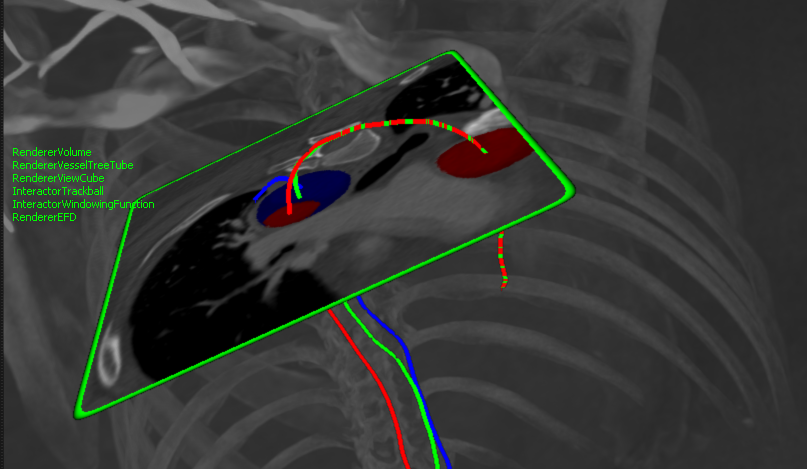
\includegraphics[width=\textwidth]{obliqueSliceOverlapping.PNG}
		
	\caption{}	
\label{fig:overlappingCase}	
	\end{subfigure}
	\begin{subfigure}[t]{0.45\textwidth}
		\includegraphics[width=\textwidth]{328_not_zoomed.PNG}
			
\caption{}	
\label{fig:overlappingCrossection}	
	\end{subfigure}
\centering
\hspace{0.08\textwidth}
\begin{subfigure}[t]{0.45\textwidth}
		\includegraphics[width=\textwidth]{328_zoomed.PNG}		
\caption{}	
\label{fig:overlappingCrosssectionZoomed}
	\end{subfigure}
	\caption{\textbf{(a)} Appearance of the TL at two different positions in the cross-sections due to high curvature of the centerline. \textbf{(b)} The cross-section obtained from (a) confuses the contour-tracing algorithm as it is not clear which of the two TL in the cross-section is the correct one. \textbf{(c)} The cross-section after applying a zooming factor. The contours are now extracted correctly.}
\label{fig:overlapping}
\end{figure}


\textbf{Distortion of lumen} 

Lumen can appear distorted within the cross-sections. Each cross-section is oriented orthogonal to the centerline that was used to obtain them. However, they are not oriented orthogonal to other centerlines. If a cross-section is not oriented orthogonal to the centerline of a lumen, the lumen appears elongated in the cross-section, because the diameter of the lumen in direction of the cross-section is larger than in the direction orthogonal to the centerline of the lumen. This is illustrated in Figure \ref{fig:cross-section_distortion}. This means that when we use the TCL to obtain cross-sections, the cross-sections are not oriented orthogonal to the centerlines of the FL and TL and both lumen may appear elongated. If we use the TL centerline, the cross-sections are not orthogonal to the FL centerline and the FL may appear elongated. If we use the FL centerline, the cross-sections are not orthogonal to the TL and the TL may appear elongated. Elongated contours are problematic because they make estimation of the lumen size difficult. Also, an elongated lumen can mean that the used step size is too large to appropriately sample the elongated lumen, resulting in a loss of features of the elongated lumen.

Currently we do not solve or avoid this problem. We do not estimate the size of the lumen. We assume that the lumen surface can be more accurately reconstructed by using the centerline of the lumen that is to be reconstructed than when using any other centerline. We also assume that the TCL is the second best choice for reconstruction: Since the TCL interpolates points that lie between the other centerlines, the angle between cross-sections obtained from the FL centerline and cross-sections obtained from the TL centerline should also be interpolated by cross-sections obtained from the TCL. This is illustrated in Figure .... 

\textbf{Choosing of the Centerline}

As we explained in the previous sections no matter which centerline we choose to obtain cross-sections at least one lumen will appear elongated in the cross-sections. For surface reconstruction we can use the centerlines of the respective lumen that is to be reconstructed for best results, but the obtained cross-sections cannot be used in all steps of the pipeline. 
When we use the TCL to obtain cross-section we only have one step size that is used while going along the spline. When we use the centerlines of the FL and TL instead, we have two different step sizes, because the step size depends on the length of the respective centerline. These differences make it complicated to use the cross-sections obtained from the centerlines of the FL and TL in some steps of the pipeline. For example in the step of the pipeline in which we correct the overlapping of the reconstructed contours we have to identify both lumen in each cross-section. In the case the cross-sections were obtained by using centerlines of the FL and TL, we can either ignore the parameter that controls the number of cross-sections to be used and process all cross-sections, or we have to decide which cross-sections to use.
The centerline of the TL is usually longer than the centerline of the FL. This means we cannot assume that the n-th cross-section of the TL is anywhere near the n-th cross-section of the FL. If we were to use only cross-sections from the FL centerline, we would not cover the whole TL. On the other hand, if we were to use only cross-sections of the TL centerline, the step size could be too large and some important features of the FL could be skipped. By using the TCL as default we avoid those problems. In case the user wants to use the respecitve lumen centerlines instead of the TCL those steps are currently skipped. An example of a cross-section obtained from the TCL can be seen in Figure \ref{fig:cross-section}.

\begin{figure}[h]
\centering
\includegraphics[width=\textwidth/2]{slice_760.PNG}
\caption{A cross-section of the phantom data set. In the center both lumen are visible. The TL is the almost perfect circular lumen with brighter intensity values than the FL. The FL is the non-circular lumen that winds arounds the TL.}
\label{fig:cross-section}
\end{figure}  

%\begin{figure}[h]
%\centering
%\includegraphics[width=\textwidth/2]{slice_760_extractedContours.PNG}
%\caption{The same cross-section as in figure \ref{fig:cross-section} after extracting the lumen contours. In the center both lumen are visible and their respective contours overlayed. The contour of the FL is colored blue, while the contour of the TL is colored red. Compared to \ref{fig:cross-section} the windowing function was adjusted for better visibility of the contours.}
%\label{fig:extracted_contours}
%\end{figure} 




\section{Extracting Lumen Contours}
\label{section:extracting_contours}
In \ref{problems_crosssections} we explained that we apply a zoom to prevent lumen to appear multiple times in the cross-section, because of the high curvature of the centerline. However, there are other reasons why a lumen can still appear multiple times in a cross-section. 

\begin{figure}
\centering
	\begin{subfigure}[t]{0.454\textwidth}
		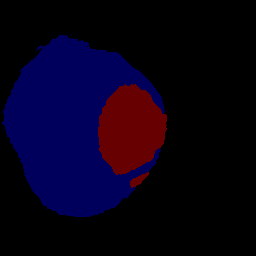
\includegraphics[width=\textwidth]{maxComponent2.png}
		\caption{}	
		\label{maxComponent}	
	\end{subfigure}
\hspace{0.13\textwidth}
	\begin{subfigure}[t]{0.4\textwidth}
		\includegraphics[width=\textwidth]{slice_760_extractedContours.PNG}
		
	\caption{}	
\label{fig:extracted_contours}	
	\end{subfigure}

	\caption{\textbf{(a)} A cross-section in which the TL appears twice despite the zoom. The TL is colored red, the FL is colored blue. \textbf{(b)} The same cross-section as in Figure \ref{fig:cross-section} after extracting the lumen contours. In the center both lumen are visible and their respective contours are overlayed. The contour of the FL is colored blue, while the contour of the TL is colored red. Compared to \ref{fig:cross-section} the windowing function was adjusted for better visibility of the contours..}
\label{fig:overlapping}
\end{figure}

An example for such a case is shown in Figure \ref{maxComponent}. In the figure the TL appears twice even after applying the zoom. In this case it probably occurs because of the way the volume data was segmented. We assume that the volume data was segmented manually by going through the slices axially. The cross-sections, however, do not generally lie in the plane of one axial slice and can therefore contain information from other axial slices. Another possibility is that this is just a case of bad segmentation.

This is the reason why before extracting the contour, we first determine the largest connected area of each lumen in the cross-section. We assume that the largest connected area in the cross-section is the real lumen from which we want to extract the contour. 

We do this by iterating over the pixels of the cross-section, left to right, top to down, until we find a pixel that belongs to a lumen. Both lumen are segmentated in our data, so we can identify pixels belonging to the lumen when traversing the cross-sections. Every time we find a non-marked pixel belonging to a lumen, we fill the area starting from the found pixel with a different color. While filling the area we count the pixels belonging to it to determine the area with the largest amount of pixels. The change in color marks the pixels and ensures that no pixel is counted more than once for each area. It also ensures that each area is only filled once. While we iterate over the cross-section pixels, we always keep track of the first pixel from the largest area we find.   

We then use the contour-tracing algorithm that we described in \ref{contourtracingalgorithm} to extract the lumen contours from the cross-sections. As a starting pixel for the contour-tracing algorithm we use the pixel from the largest area in the cross-section. In \ref{starting_pixel_conditions} we described the two conditions that the starting pixel has to fulfill. The starting pixel we use is a contour pixel and therefore satisfies the first condition. For the second condition we have to provide the inital absolute direction of the contour-tracing algorithm in a way that ensures that the left-rear pixel, relative to our starting pixel, is no inner-outer corner pixel. We set the intial absolute direction to \textit{south} to satisfy the second condition. We found the starting pixel by iterating over the cross-section pixels from left to right, top to down. This means the left-rear pixel, relative to our starting pixel, cannot be an inner-outer corner pixel. If it were an inner-outer corner pixel, it would be a contour pixel and we would have found it as the starting pixel of the area instead of the starting pixel that we actually found. The result of applying the contour-tracing algorithm is an ordered list of contour pixels and their classifications.
An example of the extracted contours can be seen in Figure \ref{fig:extracted_contours}.

\section{Converting Contour to Chain Code}
\label{section:chaincode}
In this step of the pipeline we convert the ordered list of contour pixels, which we extracted in the last step of the pipeline, into chain codes.  Specifically, we create freeman chain codes and vertex chain codes. This is done to represent the contour as a one-dimensional signal, so that we can apply the fourier transform. The chain codes are only stored temporarily and we do not use them for comparison or any other task, so we do not need to normalize them in any way. \\

\textbf{Freeman Chain Code}

We obtain the freeman chain code of a contour by iterating over the list of extracted contour pixels. For each contour pixel we compute the relative displacement to the next contour pixel and then determine which of the chain code elements shown in Figure \ref{fig:freeman} encodes the direction from the current contour pixel to the next contour pixel. We use the chain code with the 8-connectivity. \\

\textbf{Vertex Chain Code}

For the vertex chain code, we take advantage of the ability of the contour-tracing algorithm to classifiy the contour pixels. The vertex chain code encodes inner corner vertices, outer corner vertices, and straight contour segements as 3, 1, and 2 respectively. The contour-tracing algorithm can also differentiate inner corner vertices, outer corner vertices and vertices on a straight contour segment. In addition, the contour-tracing algorithm can also detect inner-outer corner vertices. The VCC does not differentiate inner-outer corner vertices because, it assumes a 4-connected contour. If the contour is 4-connected, there are no inner-outer corner vertices. However, that does not mean that an 8-connected contour cannot be encoded by an VCC. To still use the VCC for an 8-connected contour we handle inner-outer corner vertices like inner corner vertices and encode them with the chain code element 3. It should be noted that then the chain code elements do not indicate the number of cell vertices, which are in touch with the bounding contour anymore. Table \ref{vcc_table}  shows the conversation of vertex classes obtained from the contour-tracing algorithm to VCC elements. 
\begin{table}[h!]
\centering
 \begin{tabular}{c c} 
 \toprule
 Contour-Tracing Class &  VCC element\\ [0.5ex] 
 \midrule
 Inner & 3 \\ 
 Inner-outer & 3 \\
 Straight line & 2 \\
 Outer & 1 \\
\bottomrule
\end{tabular}
\caption{Conversation of the classification obtained from the contour-tracing algorithm to VCC elements.}
\label{vcc_table}
\end{table}
 
Another problem of the VCC is it's invariance to rotations as that means that the VCC only encodes the shape, not the orientation of the shape. Consequently, when a contour described by a VCC is reconstructed, the orientation of the reconstructed contour is not necessarily the same as the original contour. However, we would like to preserve the orientation of the shapes, so that when we reconstruct the lumen shapes in the volume data for visualization, the AD is orientated correctly. 

We achieve this by circulary shifting the VCC, which is the same as choosing a different starting vertex, until we find an orientation-preserving chain code element. We can identify such chain code elements, but the requirements for such chain code elements are different for counter-clockwise and clockwise VCCs.
The VCCs in our implementation always describe the contour in counter-clockwise direction. 

\usetikzlibrary{arrows.meta}
 \newcommand\VCCReconstructionOrig{
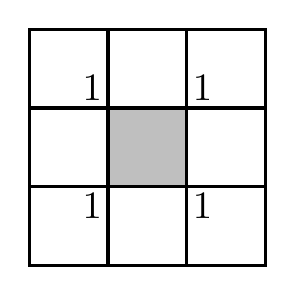
\begin{tikzpicture}
\draw [very thick, draw=black, fill=white] (0,0) grid  (3,3) rectangle (0,0);


\filldraw [fill=gray!50, draw=black, very thick] (1, 1) rectangle (2, 2);

\node[scale=1.4] (1) at (0.8, 2.25) {1};
\node[scale=1.4] (2) at (2.2, 2.25) {1};
\node[scale=1.4] (3) at (2.2, 0.75) {1};
\node[scale=1.4] (4) at (0.8, 0.75) {1};
\end{tikzpicture}
}
 \newcommand\VCCReconstructionFirst{
\begin{tikzpicture}

\draw [very thick, draw=black, fill=white] (0,0) grid  (3,3) rectangle (0,0);
\filldraw [fill=gray!50, draw=black, very thick] (1, 1) rectangle (2, 2);

\draw[draw=black, line width=2.0pt, {*[fill=darkgreen!60]}-Latex] (2, 0.85) -- (2,2);

\end{tikzpicture}
}

 \newcommand\VCCReconstructionOrigTwo{
\begin{tikzpicture}

\draw [very thick, draw=black, fill=white] (0,0) grid  (4,4) rectangle (0,0);
\filldraw [fill=gray!50, draw=black, very thick] (1, 1) rectangle (2, 2);
\filldraw [fill=gray!50, draw=black, very thick] (2, 1) rectangle (3, 2);
\filldraw [fill=gray!50, draw=black, very thick] (1, 2) rectangle (2, 3);
\filldraw [fill=gray!50, draw=black, very thick] (2, 2) rectangle (3, 3);

\node[scale=1.4] (1) at (0.8, 2.25) {2};
\node[scale=1.4] (1) at (0.8, 3.25) {1};
\node[scale=1.4] (1) at (1.8, 3.25) {2};
\node[scale=1.4] (1) at (3.2, 3.25) {1};
\node[scale=1.4] (1) at (3.2, 2.25) {2};
\node[scale=1.4] (1) at (3.2, 0.7) {1};
\node[scale=1.4] (1) at (2.2, 0.7) {2};
\node[scale=1.4] (4) at (0.8, 0.75) {1};

\draw[draw=black, line width=1.0pt, {*[fill=darkgreen!60]}-{*[fill=darkgreen!60]}] (1.85, 1) -- (3.15,1);

\end{tikzpicture}
}

 \newcommand\VCCReconstructionOrigThree{
\begin{tikzpicture}

\draw [very thick, draw=black, fill=white] (0,0) grid  (4,4) rectangle (0,0);
\filldraw [fill=gray!50, draw=black, very thick] (2, 1) rectangle (3, 2);
\filldraw [fill=gray!50, draw=black, very thick] (1, 2) rectangle (2, 3);
\filldraw [fill=gray!50, draw=black, very thick] (2, 2) rectangle (3, 3);

\node[scale=1.4] (1) at (0.8, 2.25) {2};
\node[scale=1.4] (1) at (0.8, 3.25) {1};
\node[scale=1.4] (1) at (1.8, 3.25) {2};
\node[scale=1.4] (1) at (3.2, 3.25) {1};
\node[scale=1.4] (1) at (3.2, 2.25) {2};
\node[scale=1.4] (1) at (3.2, 0.75) {1};
\node[scale=1.4] (1) at (2.2, 0.75) {1};
\node[scale=1.4] (1) at (1.8, 1.75) {3};

\draw[draw=black, line width=1.0pt, -{*[fill=darkgreen!60]}] (3,2) -- (3,0.9);
\draw[draw=black, line width=1.0pt, -{*[fill=darkgreen!60]}] (1,2) -- (2.1,2);

\end{tikzpicture}
}

 \newcommand\VCCReconstructionOrigFour{
\begin{tikzpicture}

\draw [very thick, draw=black, fill=white] (0,0) grid  (4,4) rectangle (0,0);
\filldraw [fill=gray!50, draw=black, very thick] (1, 2) rectangle (2, 3);
\filldraw [fill=gray!50, draw=black, very thick] (2, 2) rectangle (3, 3);
\filldraw [fill=gray!50, draw=black, very thick] (1,1) rectangle (2,2);

\node[scale=1.4] (1) at (0.8, 2.25) {2};
\node[scale=1.4] (1) at (0.8, 0.75) {1};
\node[scale=1.4] (1) at (0.8, 3.25) {1};
\node[scale=1.4] (1) at (1.8, 3.25) {2};
\node[scale=1.4] (1) at (3.2, 3.25) {1};
\node[scale=1.4] (1) at (3.2, 2.25) {1};
\node[scale=1.4] (1) at (2.2, 0.75) {1};
\node[scale=1.4] (1) at (2.2, 1.75) {3};

\draw[draw=black, line width=1.0pt, -{*[fill=darkgreen!60]}] (3,1) -- (3,2.1);
\draw[draw=black, line width=1.0pt, -{*[fill=darkgreen!60]}] (2,2) -- (2,0.9);

\end{tikzpicture}
}

 \newcommand\VCCReconstructionOrigFive{
\begin{tikzpicture}

\draw [very thick, draw=black, fill=white] (0,0) grid  (5,4) rectangle (0,0);
\filldraw [fill=gray!50, draw=black, very thick] (1, 1) rectangle (2, 2);
\filldraw [fill=gray!50, draw=black, very thick] (2, 1) rectangle (3, 2);
\filldraw [fill=gray!50, draw=black, very thick] (3, 1) rectangle (4, 2);
\filldraw [fill=gray!50, draw=black, very thick] (3, 2) rectangle (4, 3);
\filldraw [fill=gray!50, draw=black, very thick] (1, 2) rectangle (2,3);

\node[scale=1.4] (1) at (0.8, 2.25) {2};
\node[scale=1.4] (1) at (0.8, 0.75) {1};
\node[scale=1.4] (1) at (2.8, 3.25) {1};
\node[scale=1.4] (1) at (2.8, 2.25) {3};
\node[scale=1.4] (1) at (2.2, 0.75) {2};
\node[scale=1.4] (1) at (3.2, 0.75) {2};
\node[scale=1.4] (1) at (4.2, 0.75) {1};
\node[scale=1.4] (1) at (4.2, 1.75) {2};
\node[scale=1.4] (1) at (4.2,3.25) {1};
\node[scale=1.4] (1) at (2.2, 2.25) {3};
\node[scale=1.4] (1) at (2.2, 3.25) {1};
\node[scale=1.4] (1) at (0.8, 3.25) {1};

\draw[draw=black, line width=1.0pt, -{*[fill=darkgreen!60]}] (2,2) -- (2,0.9);
\draw[draw=black, line width=1.0pt, -{*[fill=darkgreen!60]}] (3,2) -- (3,0.9);
\draw[draw=black, line width=1.0pt, -{*[fill=darkgreen!60]}] (4,2) -- (4,0.9);

\end{tikzpicture}
}




\begin{figure}
\centering
\begin{minipage}{\textwidth}
\begin{tikzpicture}[font=\small]
\node[draw,inner sep=0pt] (c){\VCCReconstructionOrigTwo};
\node[draw,inner sep=0pt, right of=c, node distance=5cm] (f){\VCCReconstructionOrigThree};
\node[draw,inner sep=0pt, right of=f, node distance=5cm] (g){\VCCReconstructionOrigFour};
\node[draw,inner sep=0pt, below of=f, node distance=5cm] (h){\VCCReconstructionOrigFive};

\end{tikzpicture}
\end{minipage}
\caption{Different contours and their VCCs. If the VCC is counter-clockwise and one of the green vertices is used as the starting vertex, then the orientation is preserved after reconstruction.}
 \label{fig:vcc_reconstruction}
\end{figure}     

Figure \ref{fig:vcc_reconstruction} shows different contours and their counter-clockwise VCCs. The starting vertices that preserve the orientation of the contour after reconstruction are marked by green dots in the figure. If any other starting vertex is used, the contour is reconstructed rotated or mirrored. We can observe the requirements for orientation-preserving chain code elements in the figure. Note that every time the chain code element 1 is marked as an orientation-preserving starting vertex, the counter-clockwise direction the 1 encodes is upwards. Every time the chain code element 2 is marked as orientation-preserving, the encoded counter-clockwise direction is to the right. Also, every time a 3 is an orientation-preserving starting vertex, the encoded counter-clockwise direction is downwards. 

The reason why these are the requirements to preserve the orientation becomes apparent if we look at how the contour is reconstructed from the VCC. The chain code elements are first replaced by slope changes, then the integral of these slope changes is computed and it's elements are used for the equations \ref{eq:vcc_reconstruction}. Together, the equations define a direction in the unit circle. If we choose a vertex that is encoded by 1, 2, or 3 by the VCC as the starting vertex, the first element in the integral will be a $0.5$, $0$, or $-0.5$ respectively. By applying equations \ref{eq:vcc_reconstruction} on these three values, we obtain the displacements $(0, 1)$, $(1, 0)$, and $(0, -1)$. These displacements are the directions upwards, to the right and downwards, the same directions we observed for the orientation-preserving starting vertices in Figure \ref{fig:vcc_reconstruction}.

In this thesis we do not use clockwise VCCs, but for completeness we explain in the following why the requirements for clockwise VCCs are different and what these requirements are. First, it should be noted that for clockwise VCCs, no matter which starting vertex is used, the reconstruction generally has never the same orientation as the original contour. The only exception are symmetrical contours, because their counter-clockwise VCC is the same as their clockwise VCC for every starting vertex. The orientation cannot be preserved, because when the contour is traced clockwise, an outer-corner, encoded by a 1 in the VCC, can can only be traversed by rotating the direction clockwise. In the same way, an inner-corner, encoded by a 3 in the VCC, can only be traversed by rotating the direction counter-clockwise. However, the change slope values that replace a 1, and a 3 in the chain code are $0.5$, and $-0.5$ respectively. These slope change values result in a counter-clockwise, and clockwise rotation of the direction respectively, when they are added to the integral. This means that even if we try to choose an orientation-preserving starting vertex in the same way as we did for a counter-clockwise VCC, the reconstructed contour will always be at least mirrored vertically. However, we can change the slope change values to enforce a clockwise rotation for chain code element 1 and a counter-clockwise rotation for chain code element 3, for example by negating all slope change values. Then the chain code elements 1, 2, and 3 preserve the orientation of the contour, if the encoded clockwise direction is downwards, to the right, and upwards, respectively.    
 


\section{Computing Elliptic Fourier Descriptors}
In this step we compute the EFDs that will be used to represent the shapes of the lumen. As the EFDs are a set of fourier coefficients, we have to use the Discrete Fourier Transform on the chain codes we obtained in the last step of the pipeline. More specifically, we use the DFT defined in \cite{giardinia}. We described how the authors applied the fourier transform on the freeman chain code in section \ref{elliptic_fourier_descriptors}. 

In our implementation we use equations \ref{eq:dft_dc} and \ref{eq:dft_coefficients} to obtain the DC components and fourier coefficients. In \cite{giardinia} the equations were used for freeman chain codes, but theoretically they can be used for every chain code, as long as it is possible to define an euclidic length for each chain code element and a to obtain the x- and y- displacement of a chain code element. The number of harmonics is set to 10 by default, as we observed that this results in a good approximation for most lumen contours, but the value can also be freely adjusted by the user. We store the resulting EFDs, as well as the DC components, because we want to keep the translation of the contour within the cross-section, so that we can reconstruct it at the same position. Otherwise, we would not be able to reconstruct the 3D lumen shapes in the volume data for visualization correctly.

\textbf{Freeman Chain Code}

In the case the contour is described by a freeman chain code, we use equations \ref{eq:dft_dc} and \ref{eq:dft_coefficients} just as in \cite{giardinia}. Specifically, this means we also define the euclidic length of for chain elements 0, 2, 4, and 6 to be 1 and the the euclidic length chain code elements 1, 3, 5, and 7 to be $\sqrt{2}$ . The x- and y-displacements are also the same as shown in table \ref{table:freeman_displacements}.

\begin{table}[h!]
\centering
 \begin{tabular}{c c c} 
 \toprule
 Freeman Chain Code Element &  $x$-displacement & $y$-displacement\\ [0.5ex] 
\midrule
 0 & 1 & 0 \\ 
 1 & 1 & 1\\
 2 & 0 & 1\\
 3 & -1 & 1\\
 4 & -1 & 0\\
 5 & -1 & -1\\
 6 & 0 & -1\\
 7 & 1 & 1\\
\bottomrule
\end{tabular}
\caption{$x$- and $y$-displacement for each freeman chain code element.}
\label{table:freeman_displacements}
\end{table}

\textbf{ Vertex Chain Code}

In the case the the contour is a VCC we define the length of each chain code element to be 1. For the x- and y-displacements we conduct the reconstruction procedure that we described in \ref{section:vertex_chain_code}. This means we first replace the chain code elements 1, 2, and 3 by slope change values $0.5$, $0$, and $-0.5$ respectively. Then we create the integral of the slope chain values. In the last step of the reconstruction procedure, we use equations \ref{eq:vcc_reconstruction} with the values from the integral to obtain the desired x- and y-displacement for each chain code element.




\begin{figure}
	\begin{subfigure}[t]{0.45\textwidth}
		\includegraphics[width=\textwidth]{slice_760_reconstructed_1_harmonic.PNG}
	\caption{}
\label{fig:efds_reconstruction_a}		
	\end{subfigure}
\hspace{0.1\textwidth}
	\begin{subfigure}[t]{0.45\textwidth}
		\includegraphics[width=\textwidth]{slice_760_reconstructed_1_harmonic.PNG}		
\caption{}	
	\end{subfigure}
	\begin{subfigure}[t]{0.45\textwidth}
		\includegraphics[width=\textwidth]{slice_760_reconstructed_2_harmonic.PNG}
	\caption{}		
	\end{subfigure}
\hspace{0.1\textwidth}
	\begin{subfigure}[t]{0.45\textwidth}
		\includegraphics[width=\textwidth]{slice_760_reconstructed_2_harmonic.PNG}		
\caption{}	
	\end{subfigure}
	\begin{subfigure}[t]{0.45\textwidth}
		\includegraphics[width=\textwidth]{slice_760_reconstructed_5_harmonic.PNG}
	\caption{}		
	\end{subfigure}
\hspace{0.1\textwidth}
	\begin{subfigure}[t]{0.45\textwidth}
		\includegraphics[width=\textwidth]{slice_760_reconstructed_5_harmonic.PNG}		
\caption{}	
	\end{subfigure}
	\caption{}

\label{fig:efds_reconstruction}
\end{figure}

\section{Correcting of overlapping contours}
In Figure \ref{fig:efds_reconstruction} we can see that the reconstructed contours can overlap since they are just approximations of the segmented contours. The overlapping area is especially large, if a low number of harmonics is used for the reconstruction as in the first two rows of Figure \ref{fig:efds_reconstruction}. In this step of the pipeline we ensure that the reconstructed contours do not overlap. For this purpose we iterate over the cross-sections and retrieve the EFDs that describe the contours found in the corresponding cross-sections. In our implementation the EFDs are stored in a way that allows us to do so. Additionally, we can differentiate to which lumen each EFD belongs. By doing the iteration using the cross-sections we end up with two EFDs in each iteration. The first EFD describes the FL contour in the current cross-section, while the other describes the lumen contour of the TL. 
The algorithm to correct the overlapping contours can be summarized in the following five steps:

\begin{enumerate}
\item Create a layer for each lumen and draw the reconstructed contours into the corresponding layer
\item Fill the area inside the reconstructed contour
\item Combine the layers in a specific way
\item Fill each overlapping pixel with the color of the nearest contour
\item Extract contours from the result, which does not contain any overlapping contours
\end{enumerate}


\usetikzlibrary{positioning}
\usetikzlibrary{calc}

\begin{figure}
\centering
\begin{tikzpicture}



\node[inner sep=0pt, node distance=8cm] (step1_fl){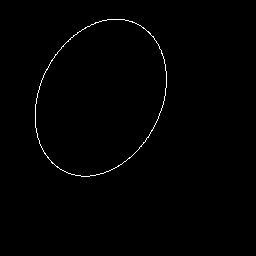
\includegraphics[width=0.3\textwidth]{/overlap_correction/step1_fl0760.png}};
\node[inner sep=0pt, right of=step1_fl, node distance=8cm, xshift=-3cm] (step1_tl){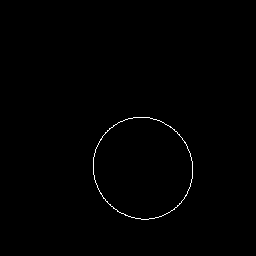
\includegraphics[width=0.3\textwidth]{/overlap_correction/step1_tl0760.png}};
\node[block, inner sep=0pt, above of=step1_fl, node distance=5cm, xshift=2.5cm] (step0) {EFDs};

\node[inner sep=0pt, below of=step1_fl, node distance=6cm] (step2_fl){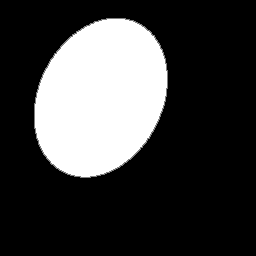
\includegraphics[width=0.3\textwidth]{/overlap_correction/step2_fl0760.png}};
\node[inner sep=0pt, below of=step1_tl,, node distance=6cm] (step2_tl){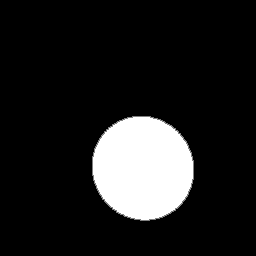
\includegraphics[width=0.3\textwidth]{/overlap_correction/step2_tl0760.png}};

\node[inner sep=0pt, below of=step2_fl, node distance=6cm, xshift=2.5cm] (step3){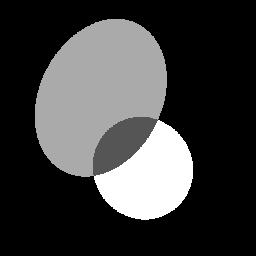
\includegraphics[width=0.3\textwidth]{/overlap_correction/step4.png}};
\node[inner sep=0pt, right of=step3, node distance=6cm] (step4){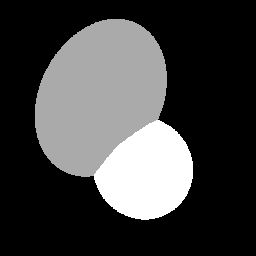
\includegraphics[width=0.3\textwidth]{/overlap_correction/step5.png}};

 \path [line, line width=3pt, -Latex] (step0) -- (step1_fl);
 \path [line, line width=3pt, -Latex] (step0) -- (step1_tl);

 \path [line, line width=3pt, -Latex] (step1_fl) -- (step2_fl);
 \path [line, line width=3pt, -Latex] (step1_tl) -- (step2_tl);

 \path [line, line width=3pt, -Latex] (step2_fl) -- (step3);
 \path [line, line width=3pt, -Latex] (step2_tl) -- (step3);
 \path [line, line width=3pt, -Latex] (step3) -- (step4);

\end{tikzpicture}
\caption{Step 1 to 4 of our overlap correction for the case shown in \ref{fig:efds_reconstruction_a}.}
\label{overlap_correction_pipeline}
\end{figure}

Figure \ref{overlap_correction_pipeline} demonstrates these first 4 steps for the case shown in \ref{fig:efds_reconstruction_a}.  
In the following we describe each of these steps in detail. 

\textbf{1. Step: Reconstruction of the contours}

In the first step we create an empty image for each of the lumen. We refer to them as \textit{layers}. Each layer has the same size as a cross-section and is initially filled with black pixels. Then we reconstruct the contours for both lumen using the EFDs.

We use the fourier approximations in equations \ref{eq:dft} to reconstruct the contours. The equations contain the variables $T$ and $t$, which are the euclidic length of the contour and the euclidic length to each chain code element respectively. However, we do not store the length of the contour and the length up to each chain code element in any step of the pipeline preceding this one. Instead, we reconstruct the contour using only the harmonics by setting $t$ to be the index of the current reconstruction point and $T$ to be the total number of reconstruction points. This changes cause the reconstructed points to be placed equidistantly on the reconstructed contour and allow the user to freely adjust the total number of reconstruction points. The main advantages of using less reconstruction points is the reduced memory consumption and faster processing due to the lower number of points that need to be processed.
 
The contour can also still be reconstructed in a gapless manner, by using enough reconstruction points. We reconstruct the contour in a gapless manner and then draw them into their corresponding layers. %The gapless reconstruction is achieved by reconstructing only a few number of contour points and then interpolate them with B-Splines. When drawing the reconstructed contours, it is important to ensure that the drawn contours can still be differentiated, for example by choosing different drawing colors / pixel intensities.%

%  We do a gapless reconstruction in the next step of the pipeline, where we fix the overlapping of the reconstructed contours. However, instead of increasing the number of %reconstructed points, we achieve a gapless reconstruction by using B-Splines to interpolate the reconstructed points. Figure \ref{fig:efds_reconstruction} shows an example of the %reconstruction for our phantom data set. On the left side of the figure are the reconstructed points. The right side of the figure shows the B-Splines that interpolate those reconstructed %points to obtain a gapless and smooth contour.  \\ 

\textbf{2. Step: Filling the inside of the contours}

In the second step, we want to fill the area inside of the contours in both layers. We use the algorithm described in \cite{inside_contour} to achieve this. The algorithm works by first creating an 4-connected external contour around the internal contour we want to fill. Then the rows that contain the contour are scanned from left to right. During this scan we have to pass the external and internal contour first, before we can reach a pixel inside the internal contour. Similarly, we know that we are leaving the inside of the internal contour when we reach a pixel belonging to the external contour after finding a pixel belonging to the internal contour. This allows us to know at all times whether we are on a pixel on the outside of the contour, on the external contour, on the internal contour or on the inside of the internal contour.

We build the external contour by using the external contour building algorithm described in \cite{inside_contour}. The contour building algorithm is basically a contour-tracing algorihm that always checks the pixel to the right of the tracer first and then checks the other pixels in the 4-neighborhood counter-clockwise. Only for the starting pixel the pixel in front of to the tracer is checked first. Since it is an contour-tracing algorihm, we have to initialize the tracer with a starting pixel position and an initial absolute directon. We obtain the starting pixel by traversing the layers, from left to right, top to down, until we find the first pixel that belongs to the reconstructed contour. The starting pixel is then the pixel above this first contour pixel. We also set the initial absolute direction to \textit{south}, so that it points to the first contour pixel.

After creating the external contour we traverse the layer once again, starting from the row below the first contour pixel that we found earlier. This row is the first row that can contain any pixels belonging to the inside of the internal contour. For every pixel we find, we check whether it belongs to the inside of the internal contour or not. If it does, we color it the same way as the reconstructed contour. The code for the scan is described by the pseudocode \ref{scan_pseudocode}.

 \begin{algorithm}
   \caption{Fill inner contour}
\label{scan_pseudocode}
    \begin{algorithmic}[1]
      \State ${StartPixel\gets}$ \textit{Starting pixel that was used for building the external contour}
        \State ${CurrentPosition\gets} (0, y$-coordinate of StartPixel $+ 2)$

\State ${FoundInternalContour\gets false}$
\State ${FoundExternalContour\gets false}$
\State ${EmptyRow\gets false}$
\State
        \While{$EmptyRow \neq true$}
\State ${CurrentPixelColor \gets }$ \textit{Pixel color at CurrentPosition}
\State
                  \If {$CurrentPixelColor = $ \textit{Color of internal contour}}
					\State ${FoundInternalContour\gets true}$
				\ElsIf{$CurrentPixelColor = $ \textit{Color of external contour}}
				\State ${FoundExternalContour\gets true}$
				\State ${FoundInternalContour\gets false}$
				\Else
					\If{$FoundInternalContour = true$}
						\State \textit{Pixel color at CurrentPosition} ${\gets}$ \textit{Color of internal contour}
					\EndIf
				\EndIf
\State
		\If{CurrentPosition = \textit{Last pixel of row}}
		\If{\textit{There is no next row or FoundExternalContour = false} }
			\State ${EmptyRow = true}$
		\Else
			\State ${CurrentPosition \gets}$ \textit{First pixel of next row}
			\State ${FoundInternalContour\gets false}$
			\State ${FoundExternalContour\gets false}$
		\EndIf
		\Else
		\State ${CurrentPosition} \gets$ \textit{next pixel of row}
		\EndIf
        \EndWhile
      


\end{algorithmic}
\end{algorithm}

\textbf{3. Step: Combining the layers}

In this step we combine both layers. We first create an image with the same size as the layers and initialize it with black pixels. For each pixel of this empty image, we check the pixels in both layers that have the same coordinates as the current pixel in the new image. By doing this we can determine if a pixel is in the overlapping region or not. More specifically, a pixel is in the overlapping region if the pixels from both layers at the same position are not black pixels. Since we initialized the layers with black pixels, all pixels that are not black belong to the corresponding lumen. If we find such a pixel, we mark the pixel at the same position in the new image by assigning a color that is different from all contour colors and not black. For all other pixels we assign their color to the pixel at the same position in the new image. We also add the pixel position of pixels, that do not lie in the overlapping region, to one of two sets that will be used in the next step. A pixel is added the first set if the pixel at the same position in the true lumen layer is not black. Similarly, a pixel is added to the second set if the pixel at the same position in the false lumen layer is not black. This means the first set contains all pixels that belong to the TL and do not lie in the overlapping region. The second set contains all pixels that belong to the FL and do not lie in the overlapping region. The new image is then the image that combines both layers. An example of such a combined image is the second last image in Figure \ref{overlap_correction_pipeline}.

\textbf{4. Step: Filling of the overlapping region}

In this step we fill the overlapping region. In the end each pixel should have the same color as the nearest pixel belonging to a lumen. However, we do not need to explicitly compute the distance of the pixel in the overlapping region to the lumen pixels. Instead, we use the wave-propagation algorithm described in \cite{porikli2007fast}. The wave-propagation algorithm works by checking the neighbors of all pixels in an \textit{active set}. The algorithm keeps track of a distance value that is increased by 1 every time a new active set is created. If a neighbor pixe that is currently checked does not have a distance value yet, it is assigned the current distance value. All pixels that get a distance value assigned are used to create a new active set. The process is repeated until no more points are in the active set.

In the paper only one active set exists, but we use the algorithm with two active sets. The initial two active sets are the two sets we created in the last step. We also do not assign a distance value to the pixels, and we do not even keep track of a distance value. In each iteration of the algorithm we first process the pixels in the active set for the TL. Each neighbor pixel that is checked and has the color that we assigned to the pixels in the overlapping region in the last step, is assigned the color of the TL. The new active set for the TL then consists of these newly colored pixels in the overlapping region. Then a do the same for the active set of the FL. We repeat the process until both active sets are empty. An example of the result can be seen in the last image of Figure \ref{overlap_correction_pipeline}.  

\textbf{5. Step: Extracting the contour}

In this last step we repeat the step of the pipeline in which we extract the lumen contours (see section \ref{section:extracting_contours}). However, this time we extract the contours from the image that we obtained after filling the overlapping regions in the 4. step of this pipeline step. We then convert the extracted contours to chain codes as we described in section \ref{section:chaincode}. Consequently, the corrected contours for both lumen are stored as chain codes. This ensures that they can be reconstructed without overlapping. 

\begin{figure}
	\begin{subfigure}[t]{0.45\textwidth}
		\includegraphics[width=\textwidth]{slice_760_reconstructed_1_harmonic_overlap_corrected.PNG}
	\caption{}		
	\end{subfigure}
\hspace{0.05\textwidth}
	\begin{subfigure}[t]{0.45\textwidth}
		\includegraphics[width=\textwidth]{slice_760_reconstructed_2_harmonic_overlap_corrected.PNG}		
\caption{}	
	\end{subfigure}
\centering
\begin{subfigure}[t]{0.45\textwidth}
		\includegraphics[width=\textwidth]{slice_760_reconstructed_5_harmonic_overlap_corrected.PNG}		
\caption{}	
	\end{subfigure}
	\caption{The reconstructed contours from Figure \ref{fig:efds_reconstruction} with corrected overlapping.}
\label{fig:obliqueslices}
\end{figure}   

\section{Generation of a Vessel Wall}
In this step of the pipeline we create an external vessel wall for rendering. Ideally, the vessel wall should fulfill the two following conditions:
\begin{enumerate}
\item{It hast to completely contain the AD}
\item{The dissection should not be visible from the outside of the vessel wall}
\label{vesselwall_conditions}
\end{enumerate}

Our vessel wall creation procedure consists of the following steps:
\begin{enumerate}
\item{Take the overlap-corrected contours from the last step of the pipeline and build several layers of external contours around them.}
\item{Compute the convex hull of the most outer layer of the external contour.}
\item{Use the points that make up the convex hull to define a periodic B-Spline.}
\end{enumerate}

\begin{figure}[t]
\centering
\begin{tikzpicture}
\node[inner sep=0pt, node distance=8cm] (step1){\includegraphics[width=0.2\textwidth]{/vesselwall/step1_0760.png}};
\node[inner sep=0pt, right of=step1, node distance=4cm] (step2){\includegraphics[width=0.2\textwidth]{/vesselwall/step2_0760.png}};

\node[inner sep=0pt, right of=step2, node distance=4cm] (step3){\includegraphics[width=0.2\textwidth]{/vesselwall/step3_0760.png}};
\node[inner sep=0pt, right of=step3, node distance=4cm] (step4){\includegraphics[width=0.2\textwidth]{/vesselwall/step4_0760.png}};

 \path [line, line width=3pt, -Latex] (step1) -- (step2);
 \path [line, line width=3pt, -Latex] (step2) -- (step3);

 \path [line, line width=3pt, -Latex] (step3) -- (step4);


\end{tikzpicture}
\caption{Alll steps of the vessel wall construction procedure for the case shown in Figure \ref{fig:efds_reconstruction_a}.}
\label{vesselwall_construction}
\end{figure}

As an example, Figure \ref{vesselwall_construction} demonstrates the vessel wall construction for the case shown in Figure \ref{fig:efds_reconstruction_a}. In the following we will describe each step of this vessel wall construction procedure in detail.

\textbf{1. Step:  Building several layers of external contours around the overlap-corrected contours}

In this step we first draw the overlap-corrected contours, that resulted in the last pipeline step, into images. Since the overlap-corected contours are stored as chain codes this is a trivial task. An example of the result is shown in the first image of Figure \ref{vesselwall_construction}. 

We then use the  external contour building algorithm described in \cite{inside_contour}, which we also used in the last step of the pipeline to build an external contour. The external contour is drawn into the same image as the overlap-contour, with the same color. This means that we cannot distinguish the external contour from the overlap-corrected contour by color anymore. Consequently, the next time we build an external contour it will be build around the previous external contour instead of around the overlap-corrected contour. We repeat building external contours and drawing them into the image $n$ times, with $n$ being the desired vessel wall thickness that can be adjusted by the user. As a result of this step we only store the last external contour that was build. In the second image of Figure \ref{vesselwall_construction} the last external contour layer is shown using a vessel wall thickness of $10$ layers.

\textbf{2. Step: Compute the convex hull}

In this step we ensure that the second condition (see \ref{vesselwall_conditions}) that the vessel wall should fulfill is satisfied. We observed that if rendered, the dissection is visible because of the ridge that appears in the surface. This ridge however, only appears because the constructed vessel wall is concave. Therefore, we decided to compute the convex hull of the last external contour. Specifically, we use the convex hull algorithm described in \cite{andrew1979another} and is implemented in the Computational Geometry Algorithms Library (CGAL) version 4.14 \cite{cgal}. 

The result of the convex hull algorithm can be seen in the third image of Figure \ref{vesselwall_construction}.

\textbf{3. Step: Approximate the convex hull by a periodic B-Spline}

In this step we use the points of the convex hull to create a periodic B-Spline. The main reason for doing this is to obtain a uniform distribution of the points that make up the vessel wall. This step is not absolutely necessary, but it prevents large regions without points in the point cloud, which could be problematic for surface recosntruction algorithms. Specifically, we use a B-Spline of degree $3$ and first create a non-periodic B-Spline using the convex hull points. It is possible to ensure that a B-Spline is periodic by adding $n$ control points, which overlap with the first $n$ control points, with $n$ being the degree of the Spline. In our case this means we add $3$ control points which are at the same positions as the first three covex hull points. We then resample the B-Spline to obtain a desired number points. In our implementation the number of points can be adjusted by the user. An example of the points of the resampled B-Spline, which is the result of this pipeline step, can be seen in the last image of Figure \ref{vesselwall_construction}.

\section{Rendering}

The result of the previous steps in the pipelines are a point cloud for the FL, TL, and for the vessel wall. In this step we use those point clouds to create a surface which can then be rendered for vessel visualization. Specifically, we use the poisson surface reconstruction \cite{kazhdan2006poisson} that is implemented in the CGAL version 4.14 \cite{cgal}. 

\begin{figure}[h]
\centering
\begin{subfigure}{0.30\textwidth}
		\includegraphics[width=\textwidth]{pointcloud_TL_zoomed.png}
	\caption{}		
	\end{subfigure}
\begin{subfigure}{0.30\textwidth}
		\includegraphics[width=\textwidth]{pointcloud_FL_zoomed.png}
	\caption{}		
	\end{subfigure}
\begin{subfigure}{0.30\textwidth}
		\includegraphics[width=\textwidth]{pointcloud_both_zoomed.png}
	\caption{}		
	\end{subfigure}

\begin{subfigure}{0.30\textwidth}
		\includegraphics[width=\textwidth]{surface_TL_zoomed.png}
	\caption{}		
	\end{subfigure}
\begin{subfigure}{0.30\textwidth}
		\includegraphics[width=\textwidth]{surface_FL_zoomed.png}
	\caption{}		
	\end{subfigure}
\begin{subfigure}{0.30\textwidth}
		\includegraphics[width=\textwidth]{surface_both_zoomed.png}
	\caption{}		
	\end{subfigure}
\caption{\textbf{(a)} Point cloud of the TL. \textbf{(b)} Point cloud of the FL. \textbf{(c)} Point cloud of the FL and TL. \textbf{(d)} Surface of the TL. \textbf{(e)} Surface of the FL. \textbf{(f)} Surface of the TL, FL, and vessel wall.}
\label{pointclouds}
\end{figure}

Figure \ref{pointclouds} shows the point clouds of each lumen and the resulting surface after applying the poisson surface reconstruction. In the Figure dual depth peeling \cite{bavoil2008order} is used to achieve the order-independent transparency of the FL, TL, and the vessel wall. 

\chapter{Results and Discussion}\label{chap:basics}
In this chapter we present the results and also evaluate the utility of the different chain codes. So far, we only used the phantom dataset to demonstrate each step of the pipeline, but for the evaluation we will use real patient data. Specifically, we will use the 3 datasets shown in Figure \ref{fig:datasets}.

\begin{figure}[h]
\centering
\begin{subfigure}{0.30\textwidth}
		\includegraphics[width=\textwidth]{dataset1.PNG}
	\caption{}		
	\end{subfigure}
\begin{subfigure}{0.30\textwidth}
		\includegraphics[width=\textwidth]{dataset2.PNG}
	\caption{}		
	\end{subfigure}
\begin{subfigure}{0.30\textwidth}
		\includegraphics[width=\textwidth]{dataset3.PNG}
	\caption{}		
	\end{subfigure}

\caption{The 3 datasets that we use for evaluation.}
\label{fig:datasets}
\end{figure}



\section{Evaluation}
In this section we describe how the utility of the chain codes is evaluated. To compare different chain codes we compute the approximation error of the chain code for each dataset by using the mean squared error (MSE), which is defined as follows: 
\begin{equation} \label{eq:mse}
 MSE = \frac{1}{n}\sum_{i=1}^{n}(Y_i - \hat{Y_i})^2
\end{equation} 
with $Y_i$ being the $ith$ point from the reconstructed contour and $\hat{Y_i}$ being the closest point to $Y_i$ out of all points from the original contour. As for parameters, we have to use a high number of cross-sections to ensure that the results are representative for the dataset. We observed that the MSE does not change significantly if we use more than 1000 cross-section, therefore we use 1000 cross-sections for each dataset. Another parameter that is of importance for the computation of the MSE is the number of harmonics that are used for the reconstruction of the contours. We observed that the MSE can change drastically if less than 10 harmonics are used. If more harmonics are used, the change is not as drastically. Therefore, we compute the MSE for 1, 2, 3, 4, 5, 6, 7, 8, 9, 10, 15, 20, 25, 30, 35, 40, 45, and 50 harmonics.
Additionally, we compare the contours, that were reconstructed using different chain codes, visually. 
\begin{table}
\centering
 \begin{tabular}{c c c c} 
 \toprule
 Dataset &  Chain Code & Number of Harmonics & MSE\\ [0.5ex] 
 \midrule
1 & Freeman & 1  & 41.700150 \\
1 & Freeman & 2  & 10.539133 \\
1 & Freeman & 3  & 4.285178  \\
1 & Freeman & 4  & 2.177701  \\
1 & Freeman & 5  & 1.522220  \\
1 & Freeman & 6  & 1.205795  \\
1 & Freeman & 7  & 1.010471  \\
1 & Freeman & 8  & 0.873905  \\
1 & Freeman & 9  & 0.781283  \\
1 & Freeman & 10 & 0.736440  \\
1 & Freeman & 15 & 0.595475  \\
1 & Freeman & 20 & 0.544211  \\
1 & Freeman & 25 & 0.514891  \\
1 & Freeman & 30 & 0.496188  \\
1 & Freeman & 35 & 0.484322  \\
1 & Freeman & 40 & 0.475767  \\
1 & Freeman & 45 & 0.469504  \\
1 & Freeman & 50 & 0.465182  \\
1 & VCC & 1  & 37.467556 \\
1 & VCC & 2  & 10.197480 \\
1 & VCC & 3  & 4.089265  \\
1 & VCC & 4  & 2.086906  \\
1 & VCC & 5  & 1.452539  \\
1 & VCC & 6  & 1.146783  \\
1 & VCC & 7  & 0.959039  \\
1 & VCC & 8  & 0.841427  \\
1 & VCC & 9  & 0.749058  \\
1 & VCC & 10 & 0.702302  \\
1 & VCC & 15 & 0.575618  \\
1 & VCC & 20 & 0.534430  \\
1 & VCC & 25 & 0.508727  \\
1 & VCC & 30 & 0.496510  \\
1 & VCC & 35 & 0.486574  \\
1 & VCC & 40 & 0.481309  \\
1 & VCC & 45 & 0.479244  \\
1 & VCC & 50 & 0.477566  \\
\bottomrule
\end{tabular}
\caption{MSE for the first dataset.}
\label{mse_1}
\end{table}

\begin{table}
\centering
 \begin{tabular}{c c c c} 
 \toprule
 Dataset &  Chain Code & Number of Harmonics & MSE\\ [0.5ex] 
 \midrule
2 & Freeman & 1  & 17.171822 \\
2 & Freeman & 2  & 5.116983  \\
2 & Freeman & 3  & 1.943756  \\
2 & Freeman & 4  & 1.214997  \\
2 & Freeman & 5  & 0.998725  \\
2 & Freeman & 6  & 0.872170  \\
2 & Freeman & 7  & 0.775425  \\
2 & Freeman & 8  & 0.722692  \\
2 & Freeman & 9  & 0.689600  \\
2 & Freeman & 10 & 0.661414  \\
2 & Freeman & 15 & 0.581981  \\
2 & Freeman & 20 & 0.544097  \\
2 & Freeman & 25 & 0.522342  \\
2 & Freeman & 30 & 0.510005  \\
2 & Freeman & 35 & 0.501772  \\
2 & Freeman & 40 & 0.497396  \\
2 & Freeman & 45 & 0.494069  \\
2 & Freeman & 50 & 0.493128  \\
2 & VCC & 1  & 15.058990 \\
2 & VCC & 2  & 4.829389  \\
2 & VCC & 3  & 1.838329  \\
2 & VCC & 4  & 1.084298  \\
2 & VCC & 5  & 0.860914  \\
2 & VCC & 6  & 0.749936  \\
2 & VCC & 7  & 0.673360  \\
2 & VCC & 8  & 0.621410  \\
2 & VCC & 9  & 0.590078  \\
2 & VCC & 10 & 0.567702  \\
2 & VCC & 15 & 0.497248  \\
2 & VCC & 20 & 0.462697  \\
2 & VCC & 25 & 0.447745  \\
2 & VCC & 30 & 0.440826  \\
2 & VCC & 35 & 0.436052  \\
2 & VCC & 40 & 0.437813  \\
2 & VCC & 45 & 0.442165  \\
2 & VCC & 50 & 0.442771 \\
\bottomrule
\end{tabular}
\caption{MSE for the second dataset.}
\label{mse_2}
\end{table}

\begin{table}
\centering
 \begin{tabular}{c c c c} 
 \toprule
 Dataset &  Chain Code & Number of Harmonics & MSE\\ [0.5ex] 
 \midrule
3 & Freeman & 1  & 41.314693 \\
3 & Freeman & 2  & 10.556674 \\
3 & Freeman & 3  & 4.198791  \\
3 & Freeman & 4  & 2.635710  \\
3 & Freeman & 5  & 1.705141  \\
3 & Freeman & 6  & 1.255415  \\
3 & Freeman & 7  & 1.046424  \\
3 & Freeman & 8  & 0.909041  \\
3 & Freeman & 9  & 0.829400  \\
3 & Freeman & 10 & 0.773351  \\
3 & Freeman & 15 & 0.627973  \\
3 & Freeman & 20 & 0.564997  \\
3 & Freeman & 25 & 0.528647  \\
3 & Freeman & 30 & 0.504973  \\
3 & Freeman & 35 & 0.490323  \\
3 & Freeman & 40 & 0.481045  \\
3 & Freeman & 45 & 0.475352  \\
3 & Freeman & 50 & 0.470534 \\
3 & VCC & 1  & 37.136673 \\
3 & VCC & 2  & 10.608171 \\
3 & VCC & 3  & 3.859052  \\
3 & VCC & 4  & 2.483811  \\
3 & VCC & 5  & 1.605258  \\
3 & VCC & 6  & 1.155338  \\
3 & VCC & 7  & 0.984269  \\
3 & VCC & 8  & 0.855931  \\
3 & VCC & 9  & 0.787047  \\
3 & VCC & 10 & 0.736885  \\
3 & VCC & 15 & 0.605078  \\
3 & VCC & 20 & 0.547484  \\
3 & VCC & 25 & 0.515092  \\
3 & VCC & 30 & 0.495841  \\
3 & VCC & 35 & 0.485159  \\
3 & VCC & 40 & 0.480503  \\
3 & VCC & 45 & 0.477290  \\
3 & VCC & 50 & 0.477742 \\
\bottomrule
\end{tabular}
\caption{MSE for the third dataset.}
\label{mse_3}
\end{table}

\section{Rendering Results}

In this section we shortly present the rendering results for each dataset and for different numbers of harmonics. Figure \ref{fig:dataset1}, Figure \ref{fig:dataset2}, and Figure \ref{fig:dataset3} show the rendering results for the 3 datasets shown in Figure \ref{fig:datasets}, for 1, 5, and 10 harmonics respectively.
\begin{figure}[!htb]
\centering
\begin{subfigure}{0.30\textwidth}
		\includegraphics[width=\textwidth]{/render_results/freeman/dataset_1/1_cropped.png}
	\caption{}		
\label{fig:dataset1_a}
	\end{subfigure}
\begin{subfigure}{0.30\textwidth}
		\includegraphics[width=\textwidth]{/render_results/freeman/dataset_1/5_cropped.png}
	\caption{}		
	\end{subfigure}
\begin{subfigure}{0.30\textwidth}
		\includegraphics[width=\textwidth]{/render_results/freeman/dataset_1/10_cropped.png}
	\caption{}		
\label{fig:dataset1_c}
	\end{subfigure}
\caption{The rendering results for the first dataset with 1, 5, and 10 harmonics.}
\label{fig:dataset1}
\end{figure}
\begin{figure}[!htb]
\centering
\begin{subfigure}{0.30\textwidth}
		\includegraphics[width=\textwidth]{/render_results/freeman/dataset_2/1_cropped.png}
	\caption{}		
	\end{subfigure}
\begin{subfigure}{0.30\textwidth}
		\includegraphics[width=\textwidth]{/render_results/freeman/dataset_2/5_cropped.png}
	\caption{}		
	\end{subfigure}
\begin{subfigure}{0.30\textwidth}
		\includegraphics[width=\textwidth]{/render_results/freeman/dataset_2/10_cropped.png}
	\caption{}		
	\end{subfigure}
\caption{The rendering results for the second dataset with 1, 5, and 10 harmonics.}
\label{fig:dataset2}
\end{figure}
\begin{figure}[!htb]
\centering
\begin{subfigure}{0.30\textwidth}
		\includegraphics[width=\textwidth]{/render_results/freeman/dataset_3/1_cropped.png}
	\caption{}	
\label{fig:dataset3_a}	
	\end{subfigure}
\begin{subfigure}{0.30\textwidth}
		\includegraphics[width=\textwidth]{/render_results/freeman/dataset_3/5_cropped.png}
	\caption{}		
\label{fig:dataset3_b}
	\end{subfigure}
\begin{subfigure}{0.30\textwidth}
		\includegraphics[width=\textwidth]{/render_results/freeman/dataset_3/10_cropped.png}
	\caption{}		
\label{fig:dataset3_c}
	\end{subfigure}
\caption{The rendering results for the third dataset with 1, 5, and 10 harmonics.}
\label{fig:dataset3}
\end{figure}

\section{Discussion}
\begin{figure}[!htb]
\centering
\begin{subfigure}{0.25\textwidth}
		\includegraphics[width=\textwidth]{/slice_results/dataset2/badExample/originalContour.PNG}
	\caption{}		
	\end{subfigure}
\begin{subfigure}{0.25\textwidth}
		\includegraphics[width=\textwidth]{/slice_results/dataset2/badExample/0_62_alone.PNG}
	\caption{}		
	\end{subfigure}
\begin{subfigure}{0.25\textwidth}
		\includegraphics[width=\textwidth]{/slice_results/dataset2/badExample/0_59_alone.PNG}
	\caption{}		
	\end{subfigure}

\begin{subfigure}{0.25\textwidth}
		\includegraphics[width=\textwidth]{/slice_results/dataset2/badExample/0_81_alone.PNG}
	\caption{}		
	\end{subfigure}
\begin{subfigure}{0.25\textwidth}
		\includegraphics[width=\textwidth]{/slice_results/dataset2/badExample/1_3_alone.PNG}
	\caption{}		
	\end{subfigure}
\begin{subfigure}{0.25\textwidth}
		\includegraphics[width=\textwidth]{/slice_results/dataset2/badExample/3_81_alone.PNG}
	\caption{}		
	\end{subfigure}

\begin{subfigure}{0.25\textwidth}
		\includegraphics[width=\textwidth]{/slice_results/dataset2/badExampleVcc/originalContour.PNG}
	\caption{}		
	\end{subfigure}
\begin{subfigure}{0.25\textwidth}
		\includegraphics[width=\textwidth]{/slice_results/dataset2/badExampleVcc/0_44.PNG}
	\caption{}
	\label{vccexcept}		
	\end{subfigure}
\begin{subfigure}{0.25\textwidth}
		\includegraphics[width=\textwidth]{/slice_results/dataset2/badExampleVcc/0_47.PNG}
	\caption{}		
	\end{subfigure}

\begin{subfigure}{0.25\textwidth}
		\includegraphics[width=\textwidth]{/slice_results/dataset2/badExampleVcc/0_56.PNG}
	\caption{}		
	\end{subfigure}
\begin{subfigure}{0.25\textwidth}
		\includegraphics[width=\textwidth]{/slice_results/dataset2/badExampleVcc/1_1.PNG}
	\caption{}		
	\end{subfigure}
\begin{subfigure}{0.25\textwidth}
		\includegraphics[width=\textwidth]{/slice_results/dataset2/badExampleVcc/3_5.PNG}
	\caption{}		
	\end{subfigure}

\caption{Reconstruction with the Freeman Chain Code (a-f) and VCC (g-l). \textbf{(a)} Original Contour \textbf{(b)} 50 Harmonics, MSR: 0.62 \textbf{(c)} 20 Harmonics, MSR: 0.59 \textbf{(d)} 10 Harmonics, MSR: 0.81 \textbf{(e)} 5 Harmonics, MSR: 1.3 \textbf{(f)} 1 Harmonic, MSR: 3.81 \textbf{(g)} Original Contour \textbf{(h)} 50 Harmonics, MSR: 0.44 \textbf{(i)} 20 Harmonics, MSR: 0.47 \textbf{(j)} 10 Harmonics, MSR: 0.56 \textbf{(k)} 5 Harmonics, MSR: 1.1 \textbf{(l)} 1 Harmonic, MSR: 3.5}
\label{fig:slice_fcc}
\end{figure}

By comparing the MSE values from Table \ref{mse_1}, Table \ref{mse_2}, and Table \ref{mse_3} we notice that the MSE for the VCC usually is lower than the MSE for the Freeman Chain Code. Looking at specific examples like the one shown in Figure \ref{fig:slice_fcc} also confirms that a contour reconstructed by a VCC usually has a lower MSE than the contour that was reconstructed using the Freeman chain code. Except for Figure \ref{vccexcept}, the VCC contours in the Figure also seem smoother than the Freeman chain code contours. However, we did not explicitly measure smoothness. Nevertheless, we measured that the VCC usually has a lower MSE than the Freeman chain code. This means that less harmonics can be used to achieve similar results. Therefore, we recommend to use the VCC instead of the Freeman chain code for this purpose.  

The rendering results in Figure \ref{fig:dataset1}, Figure \ref{fig:dataset2} and Figure \ref{fig:dataset3} show why using EFDs to model ADs is an improvement to the current state of the art. In Figure \ref{fig:dataset1_a} only one harmonic was used. Therefore, it corresponds to the current state of the art of modeling vascular structures with ellipses. However, in \ref{fig:dataset1_a} the surface was reconstructed incorrectly, because in this case the ellipse was not able to capture that the FL envelops the TL. Figure \ref{fig:dataset1_c} shows the same case, but by using 10 harmonics, the envelopment of the TL by the FL was captured and the surface was reconstructed correctly. 

\chapter{Conclusion and Future Work}\label{chap:basics}

In this thesis we demonstrated how EFDs can be used to model an AD. The results are promising and show that EFDs are an improvement to the modeling of vascular structures by ellipses. We also tested two different chain codes to represent the contour and determined that the VCC has some advantages to the Freeman chain code. 

However, we also encountered several problems that could be changed in future works. One of them is the surface reconstruction algorithm that we used. The algorithm was not able to reconstruct a surface in many cases. The surface reconstruction also is sometimes inaccurate, which can be seen in Figure \ref{fig:dataset1_c}. In the Figure the vessel wall surface intersects the FL, even though all points from the vessel wall point cloud are outside the lumen.

Another improvement, could be made to the overlap correction to better prevent gaps between the TL and FL. We observed that such gaps can occur after reconstruction from EFDs if the FL envelops the TL. In the rendering results these gaps looks like distracting shadows on the inside of the lumen. They are visible because of the transparency for example in Figure \ref{fig:dataset3_a}, and Figure \ref{fig:dataset3_b}.

A straightforward future work could be to also measure the smoothness of the reconstructed contours.  

\subfilebib % Makes bibliography available when compiling as subfile
\end{document}